\Chapter{Megvalósítás}

%Ez a fejezet mutatja be a megvalósítás lépéseit.
%Itt lehet az esetlegesen előforduló technikai nehézségeket említeni.
%Be lehet már mutatni a program elkészült részeit.
%Meg lehet mutatni az elkészített programkód érdekesebb részeit.
%(Az érdekesebb részek bemutatására kellene szorítkozni.
%Többségében a szöveges leírásnak kellene benne lennie.
%Abból lehet kiindulni, hogy a forráskód a dolgozathoz elérhető, azt nem kell magába a %dolgozatba bemásolni, elegendő csak behivatkozni.)

\Section{Kezdetek}
Még a téma megfogalmazása előtt eldöntöttem, hogy a szakdolgozatomhoz tartozó programot C\# nyelven fogom írni. Ennek legfőbb oka az eddig megszerzett nyelvi jártasságom. Magát a nyelvi verziót és a program alatt futó keretrendszert viszont a feladathoz igazítottam. Először a .NET Core 5 lett kiválasztva de kényelmi okokból, illetve mivel a platformfüggetlenség nem volt elsődleges szempont ezért  a .NET 4.7.2-es verziója lett a projekt keretrendszere. Egy érdekes tapasztalat, hogy a NuGet pkg-ket legtöbbször nem sikerül a fejlesztőknek egy éven belül frissíteni, ezért sokszor nem célszerű az éppen legfrissebb .NET verziót használni. (A kívánt pkg-k frissülése után a projekt is .NET 4.8-ra lett migrálva.) A NuGet a C\# csomagkezelője. Már megírt modulok találhatóak rajta, melyek között van ingyenes és licenszelhető is. A C\# alatt elérhető leggyakrabban használt fő alkalmazástípusok, a(z):
\begin{itemize}
\item ASP Web projekt és a hozzá választható front-end\\
\item Windows Console alkalmazás (Főként utility projektekhez használják)
\item Windows Forms "klasszikus" ablakos alkalmazás gombokkal és textboxokkal. (Leginkább a kétezres évek formavilága)
\item WPF (Windows Presentation Forms) Az előző egy "felújított" változata. Ez lényegesen több opciót biztosít a felhasználói felület testreszabására.
\end{itemize}

A projektválasztás a Windows Forms alkalmazástípusra esett. (továbbiakban WF) A WF ugyan csak egyszerű grafikai megjelenítést tesz lehetővé, de egy gráf, vagy háló folyamatai könnyedén megjeleníthetőek. A WF cserébe könnyebben szerkeszthető mint egy WPF XAML nyelven leírt felülete, és kevesebb erőforrást is igényel. 
\newpage
\Section{Fejlesztői környezet}
\subsection{Rövid történeti háttér}
A nyelvválasztás részben együtt jár a fejlesztőkörnyezet választásával is. A legelterjedtebb nyelvek mellé társul legalább egy kimondottan a nyelvhez fejlesztett fejlesztői környezet (IDE) is. A C\# -hoz ajánlott és tervezett  IDE a Visual Studio. Ennek legfrissebb kiadása a 2019-es. Eredetileg a Microsoft az általa kiadott nyelvekhez külön-külön fejlesztőkörnyezetet hozott létre, ám hamar kiderült, ez mind gazdaságilag, mind befektetett időben nem kifizetődő. Ezért először házon belül elkezdtek egy kombinált IDE fejlesztését, majd greenlight után kiadásra is áttervezték. Ez lett a Visual Studio 97. A '97-es verzió a C++, J++ és VisualBasic nyelveket támogatta natívan. A következő kiadás megtörte a később visszavezetett évszám rendszerű elnevezést és "csak" 6.0-lett. A kiadás mérföldkő volt, ugyanis ekkor jelent meg a .NET platform, aminek célja az akkor még hosszútávra tervezett két Windows rendszert, a 9x-et és az NT-t. A következő kiadás a Visual Studio .NET 2002 lett. a következő kiadással együtt (2003) léteztek különálló formábban és Visual Studio 6.0 alá tölthető modulként is. (Így nem kellett külön telepíteni egy új IDE-t és újra beállítani egy auto-deploy rendszert.) A 2002-es kiadás mutatta be a C\# nyelvet a nagyközönség számára. A C\# lényegében az akkor a SUN kezében lévő JAVA nyelv helyetteseként született. A SUN ugyanis határozatlan időre felfüggesztette a JAVA és a hozzá tartozó virtuális gép Internet Explorer alatti támogathatóságát. Eddig ugyanis, a Visual Studio a JAVA egy implementációját támogatta: a J++-t. A Microsoft a J++-t két programnyelvvel helyettesítette: a J\# -al és a C\# -al. Előbbi elég rövid életűnek bizonyult, utóbbi viszont még létezik, sőt igen elterjedtnek mondható. A C\# -ot a .NET el együtt fejlesztik, hiszen kimondottan ahhoz készült. 
Jelenleg a hagyományos .NET 4.8-as verziója a legfrissebb, de van platformfüggetlen .NET is, a .NET Core, jelenlegi nevén és kiadásán: .NET 5.

\subsection{Általános bemutatás}
A Visual Studio jelenleg három kiadása érhető el 
\begin{itemize}
\item Community 
\item Professional
\item Enterprise
\end{itemize}
A kiadások kimerítő összehasonlítása a Visual Studio oldalán érhető el.\cite{vscompare} Lényegében a Community egy ingyenes verzió, csökkentett funkcionalitással, a Professional, az analóg nevű kiadásnak felel meg, ami már teljes funkcionalitást biztosít, míg az Enterprise tartalmaz olyan funkciókat, melyek nagy, összetett projektek fejlesztését könnyítik meg. Jelenleg a Visual Studio nem tartalmaz minden támogatott nyelvet gyárilag, hanem a használni kívánt modulokat telepítéskor kell megadni. Így elkerülve a fölösleges helyfoglalást.\\
Az alapfunkciók közé tartozik az editor, a debugger, illetve a verziókezelés támogatása. Az általam használt Enterprise kiadás viszont ettől jóval többet tud. A kiadásra régebben volt szükségem, viszont öröklicenszes, ezért megmaradt. Sok kényelmi funkcióval látták el. Ilyenek például az élő függőség ellenőrzés, architektúra validáció, diagram szerkesztő, stb. Az általam egyik legtöbbet használt komponens a live debugging, ami futás közben engedi a program szerkesztését és a live unit testing, ami kód írása közben ellenőrzi a unit testek eredményét, és a kód teszt lefedettségét. Debug közben sokat segít a valós idejű memória térkép is. Itt megtekinthető a program memóriahasználata, ami lebontható a különböző modulok memória igényeire is. Továbbá a historical és snapshot debugging engedi az egy debug szálon nem előfordult, lehetséges scenario-k memória, és CPU igényének megtekintését, és a különböző esetek egymás melletti futtatását egy debug session alatt. 

\Section{Felépítés}
A fejezet elején elmondottak alapján a projektet csak 4.7.2-es .NET alatt lehetett létrehozni. A projekt eredetileg egy TDK-hoz készült, később viszont módosítva lett. Az alkalmazás felépítése a következő: 

\begin{figure}[h!]
\centering
\includegraphics[scale=0.6]{images/scheme.png}
\caption{Az alkalmazás vázlatos felépítése}
\label{fig:scheme}
\end{figure}

\textbf{FileManager / Parser } Feladata az XML file beolvasása, és tagolása. Az így feldolgozott adat kerül átalakításra a program későbbi szakaszában.\\
\textbf{Converter} A program fő része. Feladata a már tagolt adathalmaz átalakítása. Az átalakított adathalmaz DLV formátumba kerül, majd gráfleíró nyelvre. (DOT) Az így előállított háló menthető egy fileba.\\
\textbf{Display} Megjelenítő modul a konvertált háló UI-ra rajzolásáért felelős. Kis háló esetén az animáció is lehetséges.\\
\textbf{Analyzer} A hálón végezhető elemzéseket végzi el. Majd ezek eredményét megjeleníti, illetve elmenti. 

\subsection{FileManager / Parser }
A File manager a C\# hagyományos XML megoldásait használja, ez az \textbf{XmlDocument} és \textbf{XmlReader} osztály illetve a hozzá tartozó metódusok. A felhasználói felületen a felhasználó által kiválasztott file kerül a managerbe. A C\# támogatja az XML fileok hagyományos XPath alapú feldolgozását, azonban elérhető egy gyorsabb XML feldolgozás LINQ-val. A LINQ a C\# nyelvbe integrált query nyelv. Szintaktikája az SQL éhez hasonló annyi különbséggel, hogy a 'SELECT' a query végére kerül az eleje helyett. Ez főként a kódban előforduló lekérdezések elkülönülése miatt lett így tervezve. A LINQ része továbbá a Lambda expression parser is, ami hasonló lekérdezéseket tud generáli, illetve feldolgozni. 
A forrásfile beolvasása és feldolgozása kicsit bonyolultabb, mint egy sima adat XML, hiszen az adat XML nem lehet tetszőleges mély. A BPEL ezzel ellentétben elvileg igen, viszont az ilyen file olvasása több szempontból is nehézkes. Egyrészt rekurziót kell alkalmazni, ami ha nem vigyázunk nagyon hamar tele szemeteli a memóriát, illetve okozhat futásidejű hibákat is, ha például nem olyan elem van a legmélyebb szinten, mint amit vár, például sima szöveg valamilyen element helyett. BPEL során annyi könnyítést meg lehet tenni, hogy a tetszőleges mélységet előtte elhagyom, és invoke-okkal saját processen belül generálok egy új sequence-t. Az így kapott file maximum 3 szint mély lehet (a rootot leszámolva). Ezt a funkciót nem építettem bele a programba, hiszen akkor kétszer kéne végig menni ugyan azon a forrás file-on.
Ez a programban a következő kép néz ki (a következő oldalon):
\newpage
\begin{landscape}
\begin{cpp}
  XmlDocument bpelSource = new XmlDocument();
            bpelSource.Load(openFileDialog.FileName);
            XmlElement root = bpelSource.DocumentElement;
            Process process = new Process();
            process.name = root.GetAttribute("name"); 
            List<Sequence> sequences = new List<Sequence>();
            var sequenceNodes = root.ChildNodes.Cast<XmlNode>().Where(x => x.Name.Contains("sequence")).ToList();
            foreach (XmlElement item in sequenceNodes)
            {
                var childs = item.ChildNodes;
                List<BpelElement> bpelElements = new List<BpelElement>();
                foreach (XmlElement child in childs)
                {
                    var bpelElement = new BpelElement();
                    if (child.HasChildNodes)
                    {
                        foreach (XmlElement innerChild in child.ChildNodes)
                        {
                            var innerElement = new BpelElement();
                            foreach (XmlAttribute attribute in innerChild.Attributes)
                            {
                                innerElement.attributes[attribute.Name] = attribute.Value;
                            }
                            bpelElement.ownBpelElements.Add(innerElement);
                        }
                    }
                    foreach (XmlAttribute attribute in child.Attributes)
                    {
                        bpelElement.attributes[attribute.Name] = attribute.Value;
                    }
                    if (!string.IsNullOrEmpty(child.InnerText))
                    {
                        bpelElement.attributes["innerText"] = child.InnerText;
                    }
                    bpelElements.Add(bpelElement);
                }
                sequences.Add(new Sequence(item.GetAttribute("name"),bpelElements));
            }
            process.bpelSequence = sequences;
\end{cpp}
\end{landscape}
\subsection{Converter}
A Converter a program fő modulja. A leképzés fejezetben felsorolt nyelvi elemeket dolgozza fel és készíti el a részhálókat, amiket aztán összefűz. Konverzió során az XML soronként kerül feldolgozásra. Egy átolvasás után a nem szorosan illeszkedő részek, mint részhálók, segéd folyamatok stb. külön szálak kerülnek feldolgozásra aszinkron módon. Ezzel a konverziós idő (a modelltől függően) rövidül. A konverzió gyakorlatilag egy keresés egy Dictionaryben. A Dictionary egy kulcsot vár ami alapján egy értéket ad vissza. (Pont, mint egy valós szótár, ahol a kulcs az idegen nyelvű szó, az érték pedig a szó magyar megfelelője). Egy kisebb méretű Dictionary keresés durván $O(n)$ , ha $n$ darab elemre keresünk, ugyanis a \texttt{Dictionary.Contains()} egy elemre $O(1)$ komplexitású. Keresés után ezeket még rendezni kell és összefűzni. Ez utóbbi szintén minden elemre végbemegy, de ve egyidejűleg egy validáció is. A konverzió során az XML elem attribútumai és gyerekei alapján kerül az elem a háló egy adott pontjára. Ez egy újabb $O(n)$ lépés. Ha a rész szálak kész vannak és a fő szál is elkészült a részek egy hálóba lesznek rendezve ami $O(s)$, ahol az $s$ a részhálók száma. Idáig a program tehát $O(2n+s)$ lépést tesz meg. 
\subsection{Analyzer}
Az analyzer feladata az ötödik %MAKE IT REF!!!!!
 fejezetben leírtak gyakorlati alkalmazása az elkészült hálóra. Az analyzer eredetileg pythonban lett megírva. Ezt az indokolta, hogy az akkori alapalkalmazáshoz külön készült, mintegy kiegészítőként. Később a programba integrálva lett. Először IronPython alatt került bele, később teljesen átírva AGLIB-hez, majd még egyszer átírva jelenlegi Google OR toolset leírónyelvre. Az IronPython a python nyelv .NET-en futó implementációja. Gyakorlatilag kicsit gyorsabb a hagyományos pythonnál de cserébe a platform-függetlenséget feláldozza. (Jelenleg viszont az új .NET verzió futtatható Linux és MacOS rendszeren is.) Az AGLIB egy analitikus csomag aminek csökkentett képességű verziója elérhető a NuGet rendszerén keresztül ingyen. (A teljes verzió viszont licenszköteles.) A jelenleg használt Google OR tools egy ingyenesen elérhető open source software csomag optimalizáláshoz,LP, CP programozáshoz, illetve útválasztásos és flow feladatok megoldásához. A csomag előnye a felépítésében rejlik. A probléma leírása után egy proto állomány  készül, amit egy solver fog megoldani. A solver LP problémáknál a GLOP, de külső solver is használható. A solverek implementáltak több platformra is. Az elérhetőség és a független problémaleírás eredménye, hogy az OR tools támogatott C++, C\# , JAVA és Python nyelven is.
 
\subsection{Kezdeti nehézségek}
Miután körvonalazódott a feladat megvalósításának menete, létre hoztam egy kanban táblát a fejlesztési folyamatok nyomon követéséhez. (Ez a verziókezelővel együtt online, az Azure felületén érhető el.) A táblában különböző lebontásokban látható, a fő és rész egységek, valamint a feature-ök és tesztek. Az első lépés a BPEL nyelv megismerése volt. A BPEL-hez található anyagok nagy része hagyaték anyag, ugyanis a BPEL alapú folyamatkövetés kiszorult a népszerűségből. Ennek több velejárója van, de a leg szembetűnőbb, az aktívan elérhető segítség hiánya, a már hiányos dokumentáció, vagy éppen a dokumentációban felsorolt anyagok elérhetőségének hiánya. A program készítése során kellett generálni egy úgymond tanító anyagot, amely a program részeit érthetően elmagyarázza, és későbbiekben lehet használni a konverzió és a feldolgozás helyességének ellenőrzésére. Ezen tesztadatok legenerálása sokkal nagyobb nehézséget jelentett, mint vártam, vagy mint a program többi részének egy hiba utáni javítása. \\
Ismerjük meg a generáláshoz szükséges feltételeket! A BPEL írására lehet egy sima szövegszerkesztőt alkalmazni, de ez nem célravezető, mivel a háttér XML validációja kézzel nehézkesen oldható meg. A leggyakrabban hivatkozott szerkesztő az ECLIPSE. Az IDE nem támogatja alapértelmezetten a BPEL szerkesztését, ezért egy beépülő szükséges. A rendszer egy url megadása ellenében az adott szerveren tárolt beépülők letöltését, regisztrációját és integrálását teszi lehetővé. A folyamat több helyen is félre tud siklani, először az Eclipse verziójának különbözetében, aztán a szerver által alkalmazott biztonsági beállításokon, legutoljára az operációs rendszer jogosultságkezelésén. Sajnos a legfrissebb verziójú Eclipse nem támogatja a már idejét múlt szerkesztőt, ezért v6.0 körüli IDE-t kell telepíteni. A telepítés sajnos csak hagyaték rendszeren végezhető el. (ez lehet mind Linux, mind Windows). A programnak Windows 2000/Xp a rendszerkövetelménye hisz egy durván 2000-2002 es rendszerről beszélhetünk. Szerencsére a hagyaték rendszerek terén előzőleg szerzett tapasztalataim segítségemre voltak. A kettő Windows dual-boot egy korhű gépre telepítése után az editor hajlandó volt települni, egy azt megelőző gyakorlatilag verzió-hackelést követően. A frissebb Eclipse-el el kellett hitetni, hogy az állomány friss, de nem szabad volt feltelepíteni, hanem az így kinyert köteget kellett a másik gépen az Elcipse alá telepíteni manuálisan. Az IDE beállításai után lehetőség nyílt egy program szerkesztésére, de ekkor még csak validálatlan formában. Ekkor kiderült, hogy a szerkesztés befejezéséhez és validációjához egy szerverre van szükség. A szerver lehet local szerver is. A jelenleg Oracle kézben levő rendszer ehhez nem ad segítséget, de interneten található hozzá segédanyag.\cite{helloworld} Az ebből megismert Apache és ODE szerver szintén csak korhű rendszeren tud futni. A helyzetet bonyolítja, hogy a Ode-War állományokhoz jre + jvm is szükséges. A jre egy bizonyos verziója viszont inkompatibilis az ode war állomány kifejezetten ahhoz tervezett verziójával. A jre, apache tomcat, ode verziók közösen nagyon kevés működő kombinációt engednek meg. Ennek ellenére, a telepítés befejeztével a legenerált minta még mindig nem ellenőrizhető, hiszen a szervernek futnia is kell. Ellenben a futó szerverbe fel kell regisztrálni az Oracle validációs szerverét, ahonnan egy aktuális sémát vár. A letöltött séma gyakorlatilag  a BPEL verziót határozza meg. Sajnos ez a szerver 2010 óta nem működik, így a hosszadalmas munka után nem várt végeredményhez jutottam. Az így felállított rendszerrel 10 darab BPEL állományt generáltam, de mivel nagy része szerveresen állítható és kapcsolat nélkül helyfoglaló szöveg van kulcsfontosságú helyeken, így a minta felét el kellett dobni, mert szemmel láthatólag nem volt helyes. A mintagenerálást két hónap elteltével később újra megpróbáltam egy virtuális gépen ezúttal, de ekkor még kevesebb eredmény született, ugyanis az Oracle ekkor kezdte a repository-k újraszervezését. Az egy hetes átszervezés után tapasztaltam, hogy a projektet nyugdíjazták, és jelenleg sem érhető el csak a hagyaték oldalon, de tényleges letölthető forrás nélkül. A dolgozat ezen fejezetének írásakor az oldal még mindig nem elérhető. 

\subsection{A converter }
A konverzió kezelését különösen problémásnak gondoltam. Tanulmányaim során sose volt említve összetettebb adattípusok feldolgozása és azok közötti konverzió. Először egy kétszeresen összetett adattípusban gondolkoztam ami gyakorlatilag egy véges, két dimenziós tömb, hiszen a BPEL csak véges számú elemet tartalmaz gyárilag, és a szabadon definiált elemekkel nem foglalkozunk. A tömb egyik dimenziója a bejövő BPEL elem, a másik pedig a hozzá tartozó előre meghatározott konverzió eredménye. Később eszembe jutott a szakmai gyakorlat alatt szerzett információ a C\# -ban natívan jelen levő összetett adatstruktúráiról. Így esett a választás végül a Dictionary-re. A Dictionary egy 'Key - Value' azaz kulcs és érték alapon működő tár. Használata során egy kulcssort kell gyártani a rekordok számára, és a kulcshoz tartozó értéket felvinni. A Dictionary runtime, azaz futás idő alatt bővíthető ha szükséges, de mivel csak előre definiált elemeket használunk, ezért ez kihasználatlan marad. Konverzió során külön kell kezelni a színes és egyszerű Petri-hálót. Az egyszerű hálós konverzió során sokat segített Christian Stahl által közzétett publikáció\cite{bpelToPnet}.

\subsection{Vizualizáció}
A vizualizáció az alábbi módon történik:
\begin{figure}[h!]
\centering
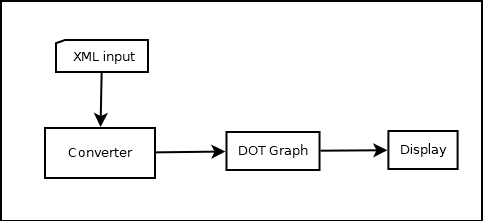
\includegraphics[scale=0.6]{images/graphdisplay.png}
\caption{A vizualizáció menete}
\label{fig:graphdisplay}
\end{figure}

A Converter előállítja a hálót, ez ekkor még nem megjeleníthető petri háló struktúrában van. Ezt a struktúrát még át kell alakítani egy Gráfrajzoló program számára is érthető formátumba. A műveletet szintén a converter végzi, ami a struktúrát tovább küldi az Analyzer számára, a gráfot pedig a rajzoló szubrutinnak. Az így kapott gráfot MS-AGL/AGLIB rajzolja ki a UI felületére. Ha a steb-by-step vizualizáció ki van kapcsolva, akkor a kirajzolt gráf a végleges. Ha viszont be van kapcsolva, akkor a tokenek fel kerülnek az ábrára és minden 1 lépés alatt lezajló művelet eredménye frissíti az adatstruktúrát. A struktúrából új kép készül, ami ki kerül a UI-ra. Ha a képeket szeretnénk elmenthetjük, ami a forrásfájl mappájába, vagy ha nincs jogosultság, akkor a program mappájába kerül mentésre. Vizualizáció során nem szükséges folyamatosnak tűnő kép előállítása, ezért használható ez a módszer. 

A program a színes háló előállításakor a forrásfájl attribútumait veszi alapul, majd figyeli, hogy egy elem hol szerepel, mik a kötődő elemei, illetve a gyerekei. Ez után egy listában szedi össze a node-ok színeit inputra és outputra. A színezés következtében a komplexitás lényegesen megnő, akár $O(n^2)$-re
